\chapter{Weather Effects on Observations}\label{chap:weather}

\vspace{-1cm}
The weather affects observations in three ways:  winds affect the telescope 
pointing, differential heating and cooling affect the telescope pointing and 
efficiency, and atmospheric opacity affect the received signal and the 
system temperature. 

\section{Winds}

Winds can set the feed arm into motion.  The current recommendations for wind limits
can be found in \S~\ref{sec:pointfocus} (specifically in Table~\ref{table:wind}).
The fraction of time when wind speeds are low is illustrated in  
Figure~\ref{fig:windspeed} which shows the cumulative percentages when 
wind speeds are below a certain value.  
(Figure~\ref{fig:windspeed} is from Ries, PTCS project Note 68.1)
The \glsfirst{DSS}, see Chapter~\ref{chap:dss}) uses forecasted wind speeds when it
determines what projects are suitable for scheduling, one should rarely see any
negative impacts from winds.

\begin{figure}[!h]
\begin{center}
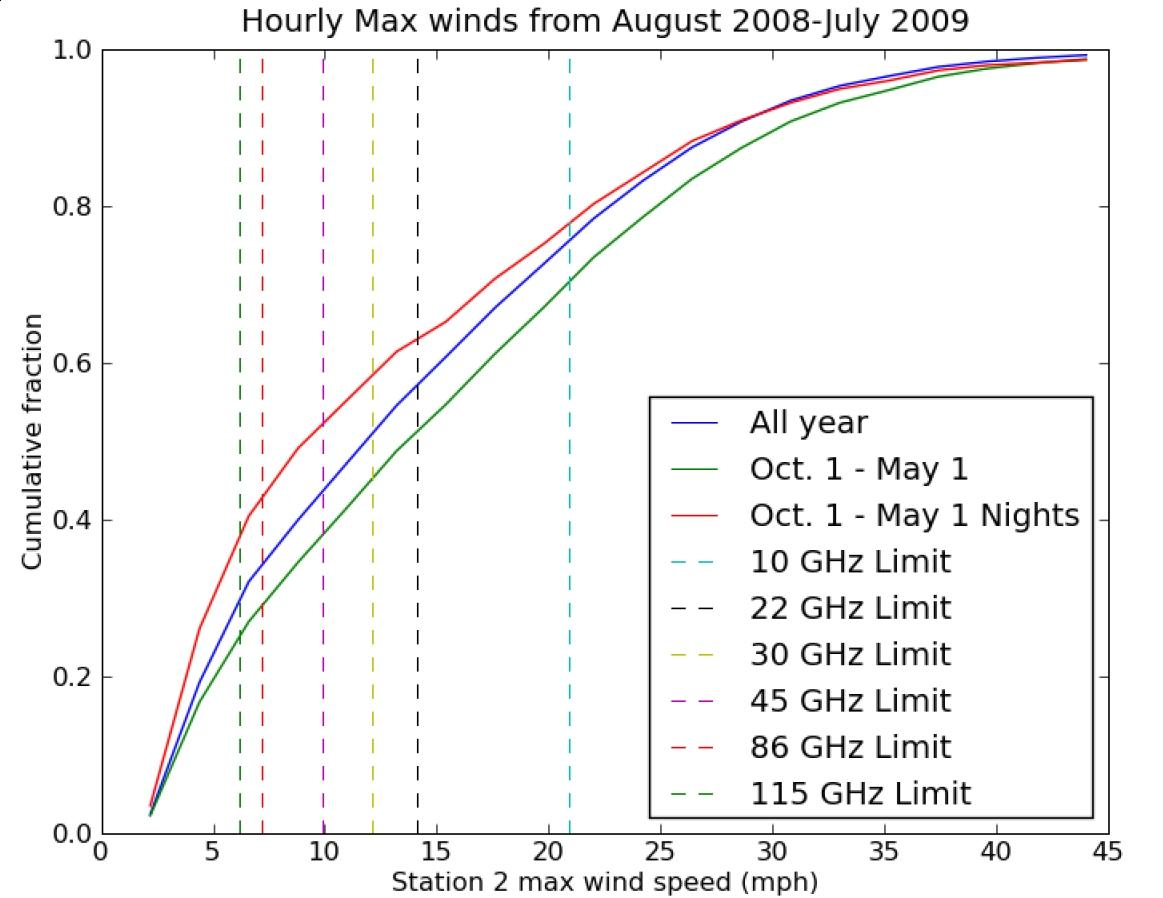
\includegraphics[width=0.65\linewidth]{windstatsfig4.jpg}
\caption[Wind speed statistics]{The cumulative fraction when wind speeds are 
below a certain value. Data from the year August 2008 to July 2009 are shown
in blue;  green shows winter data, and red shows winter nights.
%The data were for October 1, 2004 to April 30, 2005.  % Since each 
% year the weather trends can be different, these statistics shouldn't be too 
% widely quoted.  
% Note that there's very little difference between day and 
% night time wind statistics.
\label{fig:windspeed}}
\end{center}
\end{figure}

\newpage

%%%%%%%%%%%%%%%%%%%%%%%%%%%%%%%%%%%%%%%%%%%%%%%%%%%%%%%%%%%%%%%%%%%%%%%%%%%%%%
\section{Time of Day}

Differential heating and cooling of the telescope alters the surface of the 
telescope, resulting in degradation of telescope efficiencies, and \sq{bends}
the telescope, resulting in pointing changes.  At high frequencies, these 
effects are important.  The current recommendations are that, for best work, 
observing above 40~GHz should only be done at night, from 3 hours after 
sunset to 2 hours after sunrise.  At 40~GHz and above it is recommended to
use {\bfseries{\textcolor{pythonKeywords}{AutoOOF}}()} (see ~\ref{sec:AutoOOFsec}
at the start of an observing session. Use
{\bfseries{\textcolor{pythonKeywords}{AutoOOF}}} for daytime observing at
27~GHz or higher 

Low frequency observers may want to consider night time observing for two 
reasons.  \gls{RFI} is usually lower at night; and, in some cases, the sun has a 
slight negative impact on \gls{baseline} shapes.  By default, we assume that 
daytime observing will be acceptable for all observations below about 16~GHz.

Figure~\ref{fig:nighttime} depicts the range of UT, EST, and LST for our 
definition of \dq{night-time} observing. 

\begin{figure}[!h]
\begin{center}
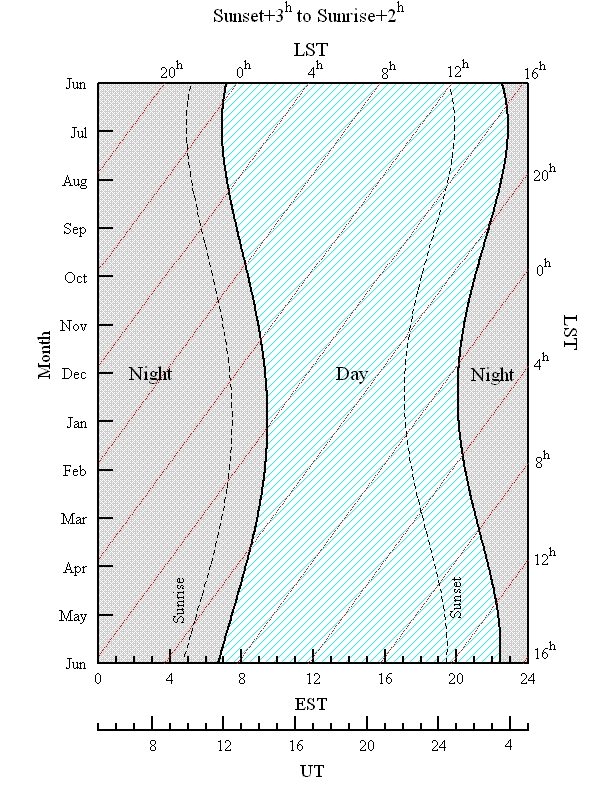
\includegraphics[width=0.75\linewidth]{SunsetSunrise2.jpg}
\caption[Night-time for the GBT]
{The range of UT, EST, and LST used in the \gls{GBT} definition for
\dq{night-time} observing.\label{fig:nighttime}}
\end{center}
\end{figure}

\newpage

%%%%%%%%%%%%%%%%%%%%%%%%%%%%%%%%%%%%%%%%%%%%%%%%%%%%%%%%%%%%%%%%%%%%%%%%%%%%%%
\section{Atmospheric Opacities}

The frequency range covered by the \gls{GBT} extends from low frequencies where 
the opacity is relatively low (~0.008 nepers) to high frequencies where opacity
is very high ($> 1$ nepers).   Atmospheric opacity hits observing twice -- it
attenuates the astronomical signal and it increases the system temperature, and
thus the noise in the observation, due to atmospheric emission.  

Figure~\ref{fig:tsysopacity} shows opacities, atmospheric contributions to the
system temperature and number of air masses\footnote{The airmass curve in 
Figure~\ref{fig:tsysopacity} is a better approximation than the csc(elevation)
approximation which is only correct above about $20^\circ$ elevation.} the
astronomical signal must pass through vs. elevation  under three typical weather
conditions as calculated using the method described on the \gls{GBT}
\dq{High Frequency Weather Forecasts} web page (\htmladdnormallink
{http://www.gb.nrao.edu/$\sim$rmaddale/Weather/index.html}
{http://www.gb.nrao.edu/~rmaddale/Weather/index.html}). Typical total system
temperatures are shown in Figure~\ref{fig:tsysweather}.

The opacities shown in Figure~\ref{fig:tsysopacity} are for planning purposes
only and observers should not use them at high frequencies for calibrating data.
Instead, one should use the actual opacities and the air mass from the bottom of
Figure~\ref{fig:tsysopacity} to approximate the amount of attenuation a signal
will experience at the expected elevation of the observation.  The signal is
attenuated by:
\begin{equation}
{\rm \exp^{\gls{tau} \gls{A}}}
\end{equation}
where \gls{tau} is the opacity and \gls{A} is the total number of air masses.
Since opacity is very weather dependent, please consult with a local support
staff on how best to determine opacities for your observing run.

During the cold months, high frequency observers can expect to be observing with
opacities that are  at or below the average (50 percentile) winter conditions for
Green Bank. Thus, high frequency observers can anticipate that the typical weather 
conditions under which they will observe will be best represented by the top 
25 percentile conditions.  In contrast, low-frequency, winter observers 
should expect they will observe under conditions that are worse than the 50 
percentile and more like those of the 75 percentile conditions.

During the warm season (June through September), high-frequency observing is 
much less productive and we almost exclusively schedule low frequency observing.
During these months, low frequency observers can plan on observing under the
average, 50 percentile conditions.

\vspace{-0.25cm}

\begin{figure}[!h]
\begin{center}
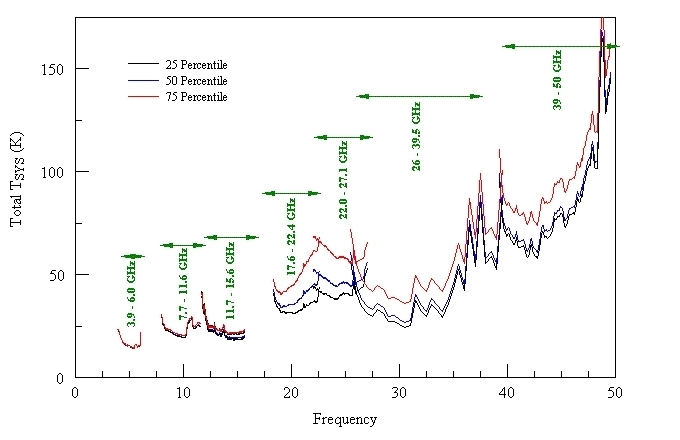
\includegraphics[width=0.7\linewidth]{TsysTotalWinter_cropped.jpg}
\caption[Typical system temperatures]
{The zenith system temperatures for typical weather conditions.
\label{fig:tsysweather}}
\end{center}
\end{figure}


\newpage

\begin{figure}[!h]
\begin{center}
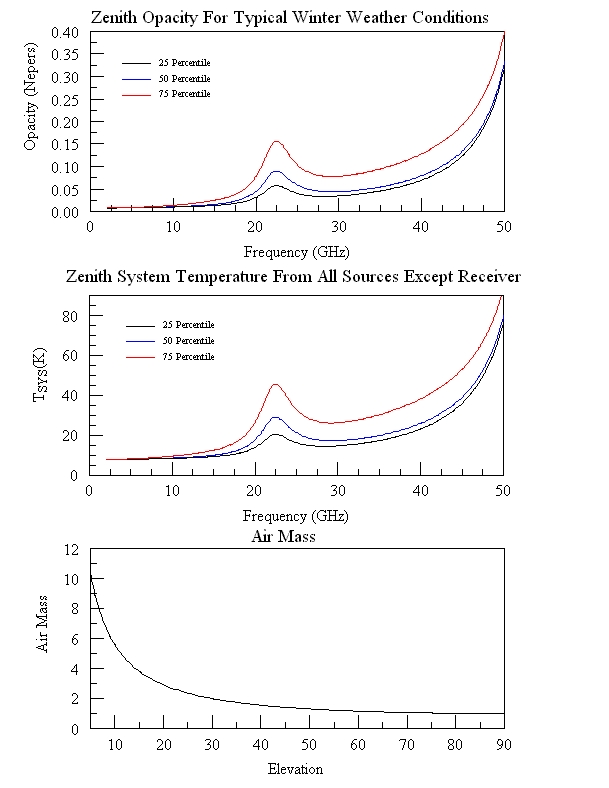
\includegraphics[width=0.9\linewidth]{TsysOpacityAirMass.jpg}
\caption[Opacity statistics]
{The top panel shows opacities under three typical weather conditions.
The black, blue, and red curves represent the opacity under the best 25, 50, 
and 75 percentile weather conditions.  (The 'average' opacity over the winter 
months is best described by the 50 percentile graph.)
The middle  panel is an estimate of the contribution to the system temperature
at the zenith from the atmosphere, spillover, and cosmic microwave background. 
The bottom panel shows the number of air masses the astronomical signal must 
pass through as a function of elevation.    
\label{fig:tsysopacity}}
\end{center}
\end{figure}

\newpage


\section{GBT Weather Restrictions}

During weather conditions that pose a risk for the safety of the GBT,
the GBT operators will cease all observations and take the appropriate
action to ensure the safety of the GBT.  The operator is fully 
responsible for the safety of the GBT and their judgement is final.
The operators decisions should not be questioned by the observer.

\subsection{Winds}

The following guidelines exist for periods of high winds.  If the 
average wind speed exceeds 35\,MPH (15.6 ms$^{-1}$) over a one minute
period, the operator will stop antenna motion.  If wind gusts exceed
40 mph (17.9 ms$^{-1}$), or if winds are expected to exceed 40 mph
for a period of time, the operator will move the antenna into the
survival position.  Only after the wind speeds have been below these
criteria for 15 minutes will observations be allowed to resume.

Safety measures for high winds will take precedence over those for
snow and ice.

\subsection{Snow}

If snow is sticking to any of the GBT structure, the operator will
move the GBT to the \dq{snow-dump} position.  The decision to halt
and resume observations is solely the responsibility of the GBT operator.

If dry snow appears to be accumulating, the operator may periodically 
interrupt operations to dump snow, and then resume observations.


\subsection{Ice}

If ice is accumulating on any part of the GBT structure, the operator will
move the GBT to the survival position.  The decision to halt
and resume observations is solely the responsibility of the GBT operator.

\subsection{Temperature}

When the air temperature drops to 16$^\circ$ Fahrenheit (-8.9\celsius),
the Azimuth slew rate of the GBT will be reduced to half of its normal
rate.  (This is due to the changing properties of the grease used in
the Azimuth drive bearings.)  Half rate speed (18$^\circ/$min instead
of 36$^\circ/$min) will be utilized until the temperature returns above
17$^\circ$ Fahrenheit (-8.3\celsius).
When the temperature drops below -10$^\circ$ Fahrenheit (-23.3\celsius)
observations will cease until the temperature is above 0$^\circ$ 
Fahrenheit (-17.8\celsius) and the operator has determined that the
Azimuth drive motors are ready for use.


\subsection{Feed Blowers}

The feed blowers blow warm air over the radomes of the feeds to 
prevent condensation and frost.  Although beneficial for most receivers,
they produce vibrations that contaminate the MUSTANG data.
Thus, users of MUSTANG can request that the operator turn off the feed blower
at the start of their observing session.  One hour before the end of a
MUSTANG observing session, the operator will decide whether or not the
blower needs to be turned back on in order to ensure the feeds for all
receivers are in good shape for the next observer.  The operators use
the criteria that the blowers will be turned back on for the last hour
if either: 1) the dew point is within 5$^\circ$ Fahrenheit of the air
temperature, or (2) the air temperature went from above to below
freezing anytime during the MUSTANG run.
